
\chapter{Real Forms of Semi-simple Algebraic Groups}\label{chap6}

In\pageoriginale this and the following sections, $G$ will denote a semi-simple
$\mathbb{R}$-groups ${}_\mathbb{R}T$ a maximal $\mathbb{R}$-split Torus,
$T$ a maximal $\mathbb{R}-$torus containing ${}_\mathbb{R}T$;
${}_\mathbb{R}\triangle$ a fundamental system of restricted roots on
${}_\mathbb{R}T$, a fundamental system of roots on $T$ whose restriction
to ${}_\mathbb{R}T$ consists of ${}_\mathbb{R} \triangle \cup \{ 0 \}$
(such a $\triangle$ can always be found). $\Phi$, $\Phi^+$ will denote
respectively the set of roots and the set of positive roots and
$\Phi^*$ the set of positive roots whose restriction to ${}_\mathbb{R}
T$ is non-zero. $\triangle_\circ$ will denote the subset of $\triangle$
consisting of those roots which are constant on ${}_\mathbb{R}T$.

Given $\alpha \in \Phi$ we define $\alpha' \in \Phi$ by the formula
 $\alpha'(\bar{x})= \overline{\alpha(x)}  \forall x \in
T$, $\bar{x}$ is complex conjugate of $x$. Then for any $\alpha \in
\triangle_\circ$ $\alpha' =- \alpha$ on $\triangle -
\triangle_\circ$. We can define a permutation $\sigma$ by
$$
\alpha' = \sigma (\alpha) + \substack{\sum n_\beta \beta\\\beta \in
  \triangle_\circ} \quad n_\beta \quad \text{non-negative integers}.
$$

\heading{Satake's Diagrams of semi-simple $\mathbb{R}-$groups.}

In Dynkin's diagram every root in $\triangle_\circ$ is denoted by a
back circle $\bullet$ and every root of $\triangle- \triangle_\circ$
by a white circle $\circ$. If $\alpha \in \triangle - \triangle_\circ$
then the white circles corresponding to $\alpha$ and $\sigma(x)$ are
joined by a arrow $\xymatrix@1{\ar@{<->}@/^/[r] &}$.

\begin{defi*}
  $G_\mathbb{R}$ is said to be $\mathbb{R}$-simple if
  $(G_\mathbb{R})^\circ$ has no proper normal subgroups of positive
  dimension. 
\end{defi*}

If\pageoriginale $G_{\mathbb{R}}$ is $\mathbb{R}$-simple, but $G$ is not
simple then $\dot {G}=$ restriction $\dot{H} = \dot{H}
\mathop{\otimes}_\mathbb{R} \mathbb{C}$, where $\dot{H}$ is a simple
Lea algebra over $\mathbb{C}/\mathbb{R}$

Thus $\dot{G}= \dot{H} \oplus \dot{H}$, and the diagram of $\dot{G}$
consists of two copies of Dynkin's diagram of $\dot{H}$, with vertices
corresponding under complex conjugation joined by arrows
%\[
%\xymatrix{0\ar@{<->}[d] \ar@{-}[r] & 0\ar@{<->}[d] \ar@{-}[r] &
%  \ar@{<->}[d] \ar@{.}[r]0- & -0\ar@{<->}[d]\\
%0 \ar@{-}[r] & 0 \ar@{-}[r] & 0- \ar@{.}[r] & -0 }
%\]

\begin{figure}[H]
  \centering{\includegraphics{figures48/fig48-0.eps}}
\end{figure}

Real forms of semi-simple Lie groups have been determined by
$F$-Gautmacher (cf. Matsbornik (47) V. 5 (1939) pp. 217-249).

The following is a complete list of $\mathbb{C}$-simple
$\mathbb{R}$-groups (cf. \cite{1}, \cite{20} \& \cite{24}).
$$
1= \sharp ~\triangle \qquad p = \sharp {}_{\mathbb{R}}\triangle
$$


\noindent 
{\fontsize{9}{11}\selectfont
\begin{longtable}{rllcl}
  & \multicolumn{1}{c}{Group} & \multicolumn{1}{c}{$\triangle$} &
  \multicolumn{1}{p{1cm}}{Type of ${}_\mathbb{R} \triangle$} &
  \multicolumn{1}{c}{$p$}\\  
  A ~I & $SL (l +1, \mathbb{R})$ &
  \includegraphics{figures48/fig48-1.eps}  & $A_1$ & $p=1$\\ 
  A II & $SU^* (l+1)$  & 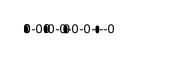
\includegraphics{figures48/fig48-2.eps} &
  $A_p$ & $p=\frac{l-1}{2}$\\[5pt]
  A III & $SU (p, q)$ &&&\\
    \multicolumn{2}{p{3cm}}{$(p < q, p+q=l+1)$} &
  \raisebox{-.5cm}{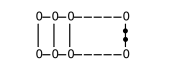
\includegraphics{figures48/fig48-3.eps}} & $B_p$ &
  $p \leq 1/2$\\[15pt]
  & $SU \left( \frac{l+1}{2}, \frac{l+1}{2} \right)$ & 
  \raisebox{-.5cm}{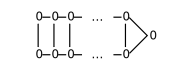
\includegraphics{figures48/fig48-4.eps}} & $C_p$ &
  $p= \frac{l+1}{2}$ \\[15pt]
  B I & $S0(p, 2l+1-p)$ &
  {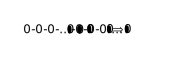
\includegraphics{figures48/fig48-5.eps}} & $B_p$ &
  $p \leq 1$\\
  C I & $S_p (n, \mathbb{R})$ &
  {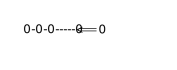
\includegraphics{figures48/fig48-6.eps}} & $C_l$ & \\
  C II & $S_p (p, l-p)$ &
  {\includegraphics{figures48/fig48-7.eps}} & $B_p$ &
  \multicolumn{1}{p{1.3cm}}{$p \leq \frac{l-1}{2}$, $l$ odd}\\
  & $S_p (l/2,l/2)$ &
  {\includegraphics{figures48/fig48-8.eps}} & $C_p$ &
  \multicolumn{1}{p{1.3cm}}{$p= l/2$, $l$ even}\\[5pt]
  D I & $S O (p, 2l-p)$ &
  \raisebox{-.3cm}{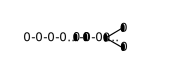
\includegraphics{figures48/fig48-9.eps}} & $B_p$ &
  \multicolumn{1}{p{1.3cm}}{$p \leq l-2$}\\
  & $SO (l.l)$ &
  \raisebox{-.3cm}{\includegraphics{figures48/fig48-10.eps}} & $D_1$ &
  \\[5pt]
  & $SO (l-1, l+1)$ &
  \raisebox{-.3cm}{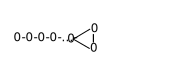
\includegraphics{figures48/fig48-11.eps}} &
  $B_{l-1}$ & \\[3pt]
  D III & $SO^*(21)$ &
  \raisebox{-.3cm}{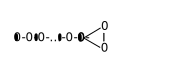
\includegraphics{figures48/fig48-12.eps}} & $B_p$ &
  $p=\frac{l-1}{2}$ \\[8pt]
  & $SO^*(21)$ &
  \raisebox{-.3cm}{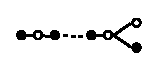
\includegraphics{figures48/fig48-13.eps}} & $C_p$ &
  $p=l/2$\\[8pt]
  & $E_6$ & \raisebox{-.3cm}{\includegraphics{figures48/fig48-14.eps}}
  & $A_2$ &\\[8pt]
  && {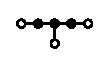
\includegraphics{figures48/fig48-15.eps}} &
  $B_2$ & \\[10pt]
  && {\includegraphics{figures48/fig48-16.eps}} &
  $E_6$ & \\[10pt]
  & $E_7$ & \raisebox{-.3cm}{\includegraphics{figures48/fig48-17.eps}}
  & $C_3$ & \\[6pt]
  & $E_7$ & \raisebox{-.3cm}{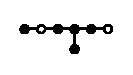
\includegraphics{figures48/fig48-18.eps}}
  & $F_4$\\[6pt]
  & $E_8$ & \raisebox{-.3cm}{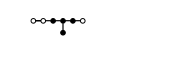
\includegraphics{figures48/fig48-19.eps}}
  & $F_4$ &\\[6pt]
  & $F_4$ & {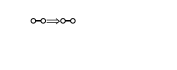
\includegraphics{figures48/fig48-20-a.eps}}
  & $F_4$ & \\
  && {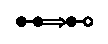
\includegraphics{figures48/fig48-20-b.eps}} &
  $\vee_1$ & \\
  & $G_2$ & {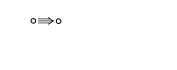
\includegraphics{figures48/fig48-21.eps}}
  & $G_2$ &
\end{longtable}}
\pageoriginale  


\begin{defi*}
  $\mathbb{R}$-rank\pageoriginale  of an algebraic group is the dimension of a
  maximal $\mathbb{R}$-split torus.
\end{defi*}

From the diagrams above, we can excerpt the diagrams of groups of
$\mathbb{R}$-rank 1 and we list the dimension of the restricted root
spaces.

Let \quad $\triangle - \triangle_\circ= \{ \alpha\}$

\noindent 
\begin{tabular}{llcc}
  \multicolumn{1}{p{5cm}}{Associated symmetric space} & diagram & $\dim
  \dot{G}_2$ & $\dim \dot{G}$\\[10pt]
  & 0 & 0 & 1\\
  Hyperbolic \Bpara{90}{0}{3600}{25} & \includegraphics{figures48/fig48-22.eps}
  & 0 & $2l-1$\\ 
  & \includegraphics{figures48/fig48-23.eps} & 0 & $2l-2$\\
  Hermitian hyperbolic & 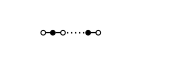
\includegraphics{figures48/fig48-24.eps} & 1
  & $2l-2$\\
  Quaternianic hyperbolic & 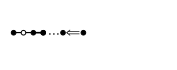
\includegraphics{figures48/fig48-25.eps} &
  3 & $4l-8$\\
  Cayley hyperbolic & 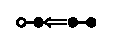
\includegraphics{figures48/fig48-26.eps} & 7 & 8
\end{tabular}

Now\pageoriginale we collect some results whose proof require examining these
diagrams.

\begin{lemma} \label{chap6:lem6.1}
  If $N$ is the set of automorophisms of $G$ stablizing $T$ and
  ${}_{\mathbb{R}}^T$, then any automorphism $\tau$ of restricted root
  system ${}_\mathbb{R}\Phi$ is induced by an element of $N$. 
\end{lemma}

\begin{proof}
  The result is true for inner automorphisms (i.e. elements in little
  Weyl group). For given any element $\sigma \in N ({}_\mathbb{R}T)$,
  both $\sigma T \sigma^{-1}$ and $T$ are contained in
  $Z({}_\mathbb{R}T)$ and therefore are maximal $\mathbb{R}$-tori of the
  connected algebraic group $Z({}_\mathbb{R}T)$. By the conjugacy of
  maximal tori, $\exists z \in Z ({}_\mathbb{R}T)$ such that
  $$
  z \sigma T \sigma^{-1} z^{-1}= T \quad \text{i.e.,}\quad z \sigma
  \in N(T)
  $$
  The inner automorphism given by $z \sigma$ is the desired element of
  $N$. 
\end{proof}

In case $\tau$, is an outer automorphism we can without loss of
generality assume that $\tau ({}_\mathbb{R}\triangle)=
{}_\mathbb{R}\triangle$.

From the usual root diagrams it is clear that only the restricted root
systems of type $A$, $E$ and $D_1$ admit an outer automorphism.

In case $A$ and $E$ the automorphism is an inner automorphism composed
with the ``opposition'' map $\alpha \mapsto -\alpha$; since each of
these extend to $\Phi$, then so does the outer automorphism.

If the restricted diagram is of type $D_l$ then the Satake diagram
shows that $\triangle= {}_\mathbb{R}\triangle$; that is the group splits
over $\mathbb{R}$ and hence the conclusion is hypothesis.

\begin{lemma} \label{chap6:lem6.2}
  If\pageoriginale $[Z({}_\mathbb{R}T), Z({}_\mathbb{R}T)]= J$ then
  $\dot{J} = \dot{J}_1 + \dot{J}_2$ is simple (possibly zero) and
  $\dot{J}_1$ is sum of compact Lie algebras of rank 1.
\end{lemma}

\begin{proof}
  We remark first that $\triangle_\circ$ is a fundamental system of
  roots for $J$. Now simply observe that the diagram of
  $\triangle_\circ$ satisfies the condition required by the conclusion.
\end{proof}

\begin{note}
  $\dot{J}_2$ is of rank 1 only if the group is $Sp(1, 2)$.
\end{note}

\begin{lemma} \label{chap6:lem6.3}
  Let $W^*$ be the subgroup of the Weyl group of $T$, which stabalizer
  ${}_\mathbb{R}T$. Then $W^*$ is irreducible on $\dot{J}_1 \cap
  \dot{T}$ and $\dot{J}_2 \cap \dot{T}$.  
\end{lemma}

\begin{proof}
  $\dot{J}_2 \cap \dot{T}$ is a cartan subalgebra of the simple Lie
  algebra $\dot{J}_2$ and, as is well known, the Weyl group of a
  simple Lie algebra operates irreducibly of its associated Cartan
  subalgebra. It remains only to prove that $W^*$ is irreducible on
  $\dot{J}_1 \cap \dot{T}$.
\end{proof}

Inspection of the position of $\triangle_\circ$ in $\triangle$, as
pictured in the diagrams shows that $\dot{J}_1$ is contained in a
subalgebra of type $A_{2p-1}$ with the diagram \quad 
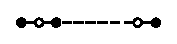
\includegraphics{figures48/fig48-27.eps}. 

As is known, the Weyl group of $A_{2 p-1} \approx SL (2p)$ is the
group of permutations of the standard basis vectors $e_1, \ldots ,
e_{2p}$ in $\mathbb{C}^{2p}$. The roots $\triangle_{\circ; 1}$ of
$\dot{J}_1$ become identified with $\{ \alpha_{2i-1}- \alpha_{2i},
i=1, \ldots p\}$ where $\alpha_i$ denotes the $i^{\text{th}}$ matrix
coefficient. Clearly the stabalizer of $\dot{J}_1$ contains the
conjugation by the matrix sending each. $e_{2i-1} \to e_{2 \pi (i)
  -1}$ and $e_{2i} \to e){2 \pi (i)}$, for any permutation $\pi$ of
$\{ 1, \ldots , p\}$. Since these automorphisms of $\dot{J}_1$ induce
the full symmetric group on the elements of the set $\triangle_{\circ,
  1}$, we conclude that $W^*$ is irreducible on $\dot{J}_1 \cap
\dot{T}$.

\begin{lemma} \label{chap6:lem6.4}
  Let\pageoriginale $G_1$, $G_2$ be two $\mathbb{C}$-simple
  $\mathbb{R}$-groups. Assume $\tau : T_1 \to T_2$ is an isomorphism
  sending ${}_{\mathbb{R}} T_1 \to {}_{\mathbb{R}} T_2$ and $\Phi^*_1 \to
  \Phi_2^*$. Then $\dot{G}_1 \approx \dot{G}_2$ and ${}^\tau|_{\mathbb{R}} 
  \dot{T}_1$ can be induced by an isomorphism of $\dot{G}_1$ and $\dot{G}_2$.
\end{lemma}

\begin{proof}
  Suppose first that $p$, the $\mathbb{R}$-rank of $G_1$ and $G_2$ is
  one. Then the $\tau$-corresponding restricted root spaces must have
  the same dimension. The listed values in our table for $\dim
  G_\alpha$ and $\dim G_{2\alpha}$ show that these determine the group
  of $\mathbb{R}$-rank 1. Thus $\dot{G}_1 \approx \dot{G}_2$ in the
  rank 1 case. Moreover, the isomorphism $\theta$ of $\dot{G}_1$ to
  $\dot{G}_2$ can be taken so as to map the restricted root spaces of
  $\dot{G}_{1, \alpha}$ of $\dot{G}_1$ to the restricted root space
  $\dot{G}_{2, \tau (\alpha)}$ of $\dot{G}_2$. It follows at once that
    $\theta$ and $\tau$ induce the same map on ${}_{\mathbb{R}}\dot{T}$ and thus
    the lemma is proved for $p=1$.
\end{proof}

Suppose now that $\sharp {}_\mathbb{R}\triangle > 1$. We need only
consider the case that the groups are not split over $\mathbb{R}$
(i.e., $\triangle \neq {}_\mathbb{R}\triangle$), otherwise the result is
a well-known theorem of Weyl. Assuming therefore that $\triangle \neq
{}_\mathbb{R}\triangle$ we find that the restricted root diagrams are of
type $A, B, C, F_4$. In neither of these cases does the Dynkin diagram
of ${}_\mathbb{R}\triangle$ have a branch point. Therefore given a
Satake diagram $\triangle$ of a non $\mathbb{R}$-split group, one can
form a sequence of the subdiagrams $\triangle^{(1)} \subset
\triangle^{(2)}\ldots \subset \triangle^{(p)} =\triangle$ such that 

\begin{enumerate}[(a)]
\item $\sharp {}_\mathbb{R} \triangle^{(k)}=k$
  \item $\triangle^{(k+1)}= \triangle^{(k)} \cap D^{k+1}$ where
    $\sharp {}_\mathbb{R} D^{k+1}=1$.
    \item $D^{k} \cap D^{k+1} = D^{k+1} \cap \triangle^{(k)}$.
\end{enumerate}

Given\pageoriginale now the two groups $G_1$ and $G_2$ and the map
$\tau$, we decompose the Satake diagram $\triangle_i$ of $G_i$ as
above, getting $\triangle_i = \triangle_i^{(p-1)} \cup D^p_i$. By
induction there are isomorphisms $\theta^{(p-1)}: \triangle_1^{(p-1)}
\to \triangle_2^{(p-1)}$ and $\theta_p : D_1^p \to D^p_2$ induced by
isomorphisms of the corresponding Lie algebras $\dot{G}_i^{(p-1)}$ and
$F_i^p$. Let $\varphi$ denote the restriction of $\theta_p^{-1} \cdot
\theta^{p-1}$ to $\dot{G}_1^{(p-1)} \cap \dot{F}_i^p$.

Set $\triangle^p_{i, \circ}= \triangle_i^{(p-1)} \cap D^p_i$. Then
$\triangle_{i, \circ}^p$ is connected since the root diagram
$\triangle$ has no loops. In fact by property $(c)$ $\triangle^p_{i,
  \circ}= D^{p-1}_i \cap D^p_i$ and is in fact a connected component
in $\triangle_{i, \circ}$, the diagram of the $\mathbb{R}$-compact
part of $Z(T_i)$. An additional inspection of the diagrams shows that
no connected component of the diagram of $Z(T_1)$ admits an (outer)
automorphisms. Hence $\varphi$ is an inner automorphisms of
$\dot{G}_1^{(p-1)} \cap \dot{F}^p_1$ and thus extends to an
automorphisms $\chi$ of  $\dot{G}_1$. Replacing $\theta_p$ by
$\theta_p \cdot \chi$, we obtain the derived isomorphisms of
$\dot{G}_1$ onto $\dot{G}_2$.

The following is an easy consequence of previous lemma.

\begin{thm} \label{chap6:thm6.5}
  Let $G$ be a semisimple $\mathbb{R}$-group having no compact
  factors. Let $\tau: T \to T$ be an isomorphism which stabilizes
  ${}_\mathbb{R} T$ and $\Phi^*$. Then there exists an automorphism
  $\theta$ of $G$ such that $\theta \cdot \tau$ stabilizes $T$ and on
  ${}_\mathbb{R} T$ it is identity. 
\end{thm}

\begin{lemma} \label{chap6:lem6.6}
  Let $G$ be a semisimple $\mathbb{R}$-group with no
  $\mathbb{R}$-compact factors. We also assume that $G_\mathbb{R}$ is
  simple of $\mathbb{R}$-rank 1. If $\tau$ is an automorphisms of $T$
  stabilizing ${}_\mathbb{R} T$ and $\Phi^*$, then it stabilizes
  $\dot{J} \cap \dot{T}$, $\dot{J}_1 \cap \dot{T}$\pageoriginale and
  $\dot{J}_2 \cap \dot{T}$.
\end{lemma}

\begin{proof}
  Let 
  $$
  B^* = \sum_{\alpha \in \Phi^*} \alpha^2
  $$
  Then $\tau$ preserves $B^*$. Let $B, B_\circ$ denote the killing
  forms of $G$ and $Z(T)$ respectively then $B= B_\circ+ 2 B^*$. So
  any two subspaces of $\dot{T}$ orthogonal with respect to both $B$
  and $B_\circ$ are orthogonal with respect to $B^*$.
\end{proof}

Let $X, X' \in \dot{J}_1$ and $Y \in \dot{J}_2$, then 
$$
B([X, X'], Y)= - B(X', [X, Y])=0
$$
and since $[\dot{J}_2, \dot{J}_2]= - \dot{J}_2$, we have $B(\dot{J}_1,
\dot{J}_2)=0$ similarly $B_\circ (\dot{J}_1, \dot{J}_2)=0$
$$
\therefore \quad B^* (\dot{J}_1 \cap \dot{T}, \dot{J
}_2  \cap \dot{T})=0.
$$

Composing $\tau$ with an automorphisms of $\dot{G}$, we can assume by
the Theorem \ref{chap6:thm6.5} that $\tau$ induces identity on
${}_\mathbb{R} T$. Thus $\tau$ stabilizes the set of all roots having
a non-trivial restriction on ${}_\mathbb{R} T$ and we can assume
accordingly that ${}_\mathbb{R} \triangle$ consists of a single
element, and that the set of positive roots in ${}_\mathbb{R} \Phi$ is
either $\{\bar{\alpha} \}$ or $\{ \bar{\alpha}, 2 \bar{\alpha}\}$. Let
$S$ denote the set of roots restricting to $\bar{\alpha} \cdot\tau$
stabilizes $\Phi^*$ and therefore also the set $S-S$ of differences of
roots in $S$. These differences clearly lie in linear span of $\{
\triangle_\circ\}$, conversely, given any root $\beta \in \{
\triangle_\circ\}$ we shall show that $\beta$ occurs in $S-S$. We can
assume $\beta > 0$. 

The\pageoriginale hypothesis that $G$ contains no $\mathbb{R}$- compact factors is
tantamount to the hypothesis that $\{G_\alpha, \pm \alpha \in S \}$
generates $G$. Hence $<\beta, S>\neq 0$. Let $\alpha$ be the least
root in $S$ for which $<\beta, \alpha>\neq 0$. Then $\sigma_\beta
(\alpha)= \alpha + q (\alpha, \beta) \beta$ is a root where $q(\alpha,
\beta)= \frac{-2 <\alpha, \beta>}{<\beta, \beta>}$ is a positive
integer. Thus $\alpha + q (\alpha, \beta) \beta \in S$ and $\beta \in
S-S$. Hence $\{S-S\}= \{ \triangle_\circ\}$ as asserted.

Therefore $\tau$ stabilizes the intersection of the kernels of the
linear functions in $\triangle_\circ$ e.g. $\tau$ stabilizes $Z(J)
\cap \dot{T}$. Now $\dot{J} \cap \dot{T}$ is the orthogonal complement
of $Z(J) \cap \dot{T}$ with respect to both killing forms $B$ and
$B_\circ$ and therefore with respect to $B^*=B-2B_\circ$. Since $\tau$
stabilizes $B^*$, it stabilizes $\dot{J} \cap \dot{T}$.

Having assumed that $G$ has $\mathbb{R}$-rank 1, we see that $\tau$ is
simple in all cases except $G= C_l (l=3)$ or $G=D_3$. In the second
case $\dot{J}= \dot{J}_1, \dot{J}_2=0$ and the Lemma is
established. In case $G= C_l(l=3)$ the diagram is 
\begin{figure}[H]
 \centering{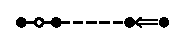
\includegraphics{figures48/fig48-28.eps}}
\end{figure}
\noindent and the roots in $\Phi^*$ having the same restriction to
${}_\mathbb{R} T$ as $2 \alpha_2$ are $2 \alpha_2 + \ldots + 2
\alpha_{l-1} + \alpha_l$; $\alpha_1 + 2 \alpha_2 + \ldots 2
\alpha_{l-1} + \alpha_1$, $2 \alpha_1+ 2 \alpha_2 + \ldots + 2
\alpha_{l-1}+ \alpha_l$. Since $\tau$ permutes this set, it permutes
the differences and therefore $\tau \alpha_1 = \pm \alpha_1$. Hence
$\tau$ stabilizes $\dot{T}_2= \ker \alpha_1 \cap \dot{J}$, and
therefore stabilizes $\dot{T}_1$ which is the orthogonal complement of
$\dot{T}_2$ in $\dot{T} \cap \dot{J}$ with respect to $B^*$. The proof
  of the Lemma is now complete.
